
\documentclass[%
 reprint,
%superscriptaddress,
%groupedaddress,
%unsortedaddress,
%runinaddress,
%frontmatterverbose, 
%preprint,
%preprintnumbers,
nofootinbib,
%nobibnotes,
%bibnotes,
 amsmath,amssymb,
 aps,
%pra,
%prb,
%rmp,
%prstab,
%prstper,
floatfix,
]{revtex4-2}
\usepackage{gensymb}
\usepackage{textcomp}
\usepackage{graphicx}% Include figure files
\usepackage{dcolumn}% Align table columns on decimal point 


\usepackage{bm}% bold math
\usepackage{siunitx}
\DeclareSIUnit\gauss{G}
\DeclareSIUnit\erg{erg}
\DeclareMathOperator{\Rot}{rot}
\sisetup{separate-uncertainty=true}
\usepackage{tabularx}
\usepackage{amssymb}
\usepackage{amsmath}
\usepackage{relsize}
\usepackage{commath}
\usepackage{enumitem}
\usepackage{float}
\usepackage{booktabs}
\usepackage{makecell}
\usepackage[version=4]{mhchem}
\usepackage[colorlinks,bookmarks=false,citecolor=blue,linkcolor=blue,urlcolor=blue]{hyperref}
%\usepackage{hyperref}% add hypertext capabilities
%\usepackage[mathlines]{lineno}% Enable numbering of text and display math
%\linenumbers\relax % Commence numbering lines

%\usepackage[showframe,%Uncomment any one of the following lines to test 
%%scale=0.7, marginratio={1:1, 2:3}, ignoreall,% default settings
%%text={7in,10in},centering,
%%margin=1.5in,
%%total={6.5in,8.75in}, top=1.2in, left=0.9in, includefoot,
%%height=10in,a5paper,hmargin={3cm,0.8in},
%]{geometry}

\begin{document}

\preprint{APS/123-QED}

\title{Electron Spin Resonance}% Force line breaks with \\


\author{Maitrey Sharma}
\email{maitrey.sharma@niser.ac.in}
\affiliation{School of Physical Sciences, National Institute of Science Education and Research, HBNI, Jatni-752050, India}




\date{\today}% It is always \today, today,
             %  but any date may be explicitly specified

\begin{abstract}
    In this experiment, we study about the phenomena of electron spin resonance, which is often used as a spectroscopic technique to identify paramagnetic materials. We discuss the Larmor precession, the $g$-factor, specially Land\'e $g$-factor and justify its appearance in our discussions. We review the classical and quantum mechanical picture of the magnetic moment of electron in paramagnetic materials. We explore the ESR phenomena in macroscopic systems like solids. We formulate the theory for the experiment and workings of the ESR spectrometer. We finally determine the Land\'e $g$-factor for the electron and finally discuss the results so obtained like the appearance of four peaks on the oscilloscope and how the obtained Lissajous figure provides the insight on the effects of external magnetic field when a paramagnetic substance is kept under its influence. In the process of this experiment, we establish various useful results relates to magnetism and behaviour of electron in magnetic fields.
\end{abstract}

\keywords{Zeeman effect, energy quantum, quantum number, resonance, $g$-factor, land\'e factor}
\maketitle

%\tableofcontents

\section{\label{sec:level1}Introduction}
    Spectroscopy, primarily in the electromagnetic spectrum, has played the role of a fundamental exploratory tool in the fields of physics, chemistry, and astronomy, allowing the composition, physical structure and electronic structure of matter to be investigated at the atomic, molecular and macro scale, and over astronomical distances since its inception. Especially in chemistry, it has been of immense importance as the combination of atoms into molecules leads to the creation of unique types of energetic states and therefore unique spectra of the transitions between these states. Molecular spectra can be obtained due to electron spin states (electron spin resonance or electron paramagnetic resonance), molecular rotations, molecular vibration, and electronic states.
    \par
    \textbf{Electron paramagnetic resonance} (EPR) or \textbf{electron spin resonance} (ESR) spectroscopy is a method for studying materials with unpaired electrons. In general, resonance implies the enhancement of the amplitude when the frequency of the externally applied force matches with the natural frequency of the system. The basic concepts of ESR are analogous to those of nuclear magnetic resonance (NMR), but the spins excited are those of the electrons instead of the atomic nuclei.
    \par
    Soviet physicist Yevgeny Zavoisky started his work on ESR in 1943 after failing to materialise his work on NMR and due to interruption from the war as it was less demanding. In 1944, ESR signals were detected in several salts, including hydrous copper chloride (\ce{CuCl2.2H2O}), copper sulfate and manganese sulfate. The results were revolutionary and were first not accepted even by the Soviet scientists (including Pyotr Kapitsa, known for his work on superfluidity). The doubts were dispersed when Zavoisky visited Moscow, assembled an ESR spectrometer from scratch and reproduced his results there. In 1945, Zavoisky defended his habilitation on the phenomenon of electron spin resonance. ESR was also developed independently around the same time by Brebis Bleaney at the University of Oxford.
    \begin{figure*}
        \centering
        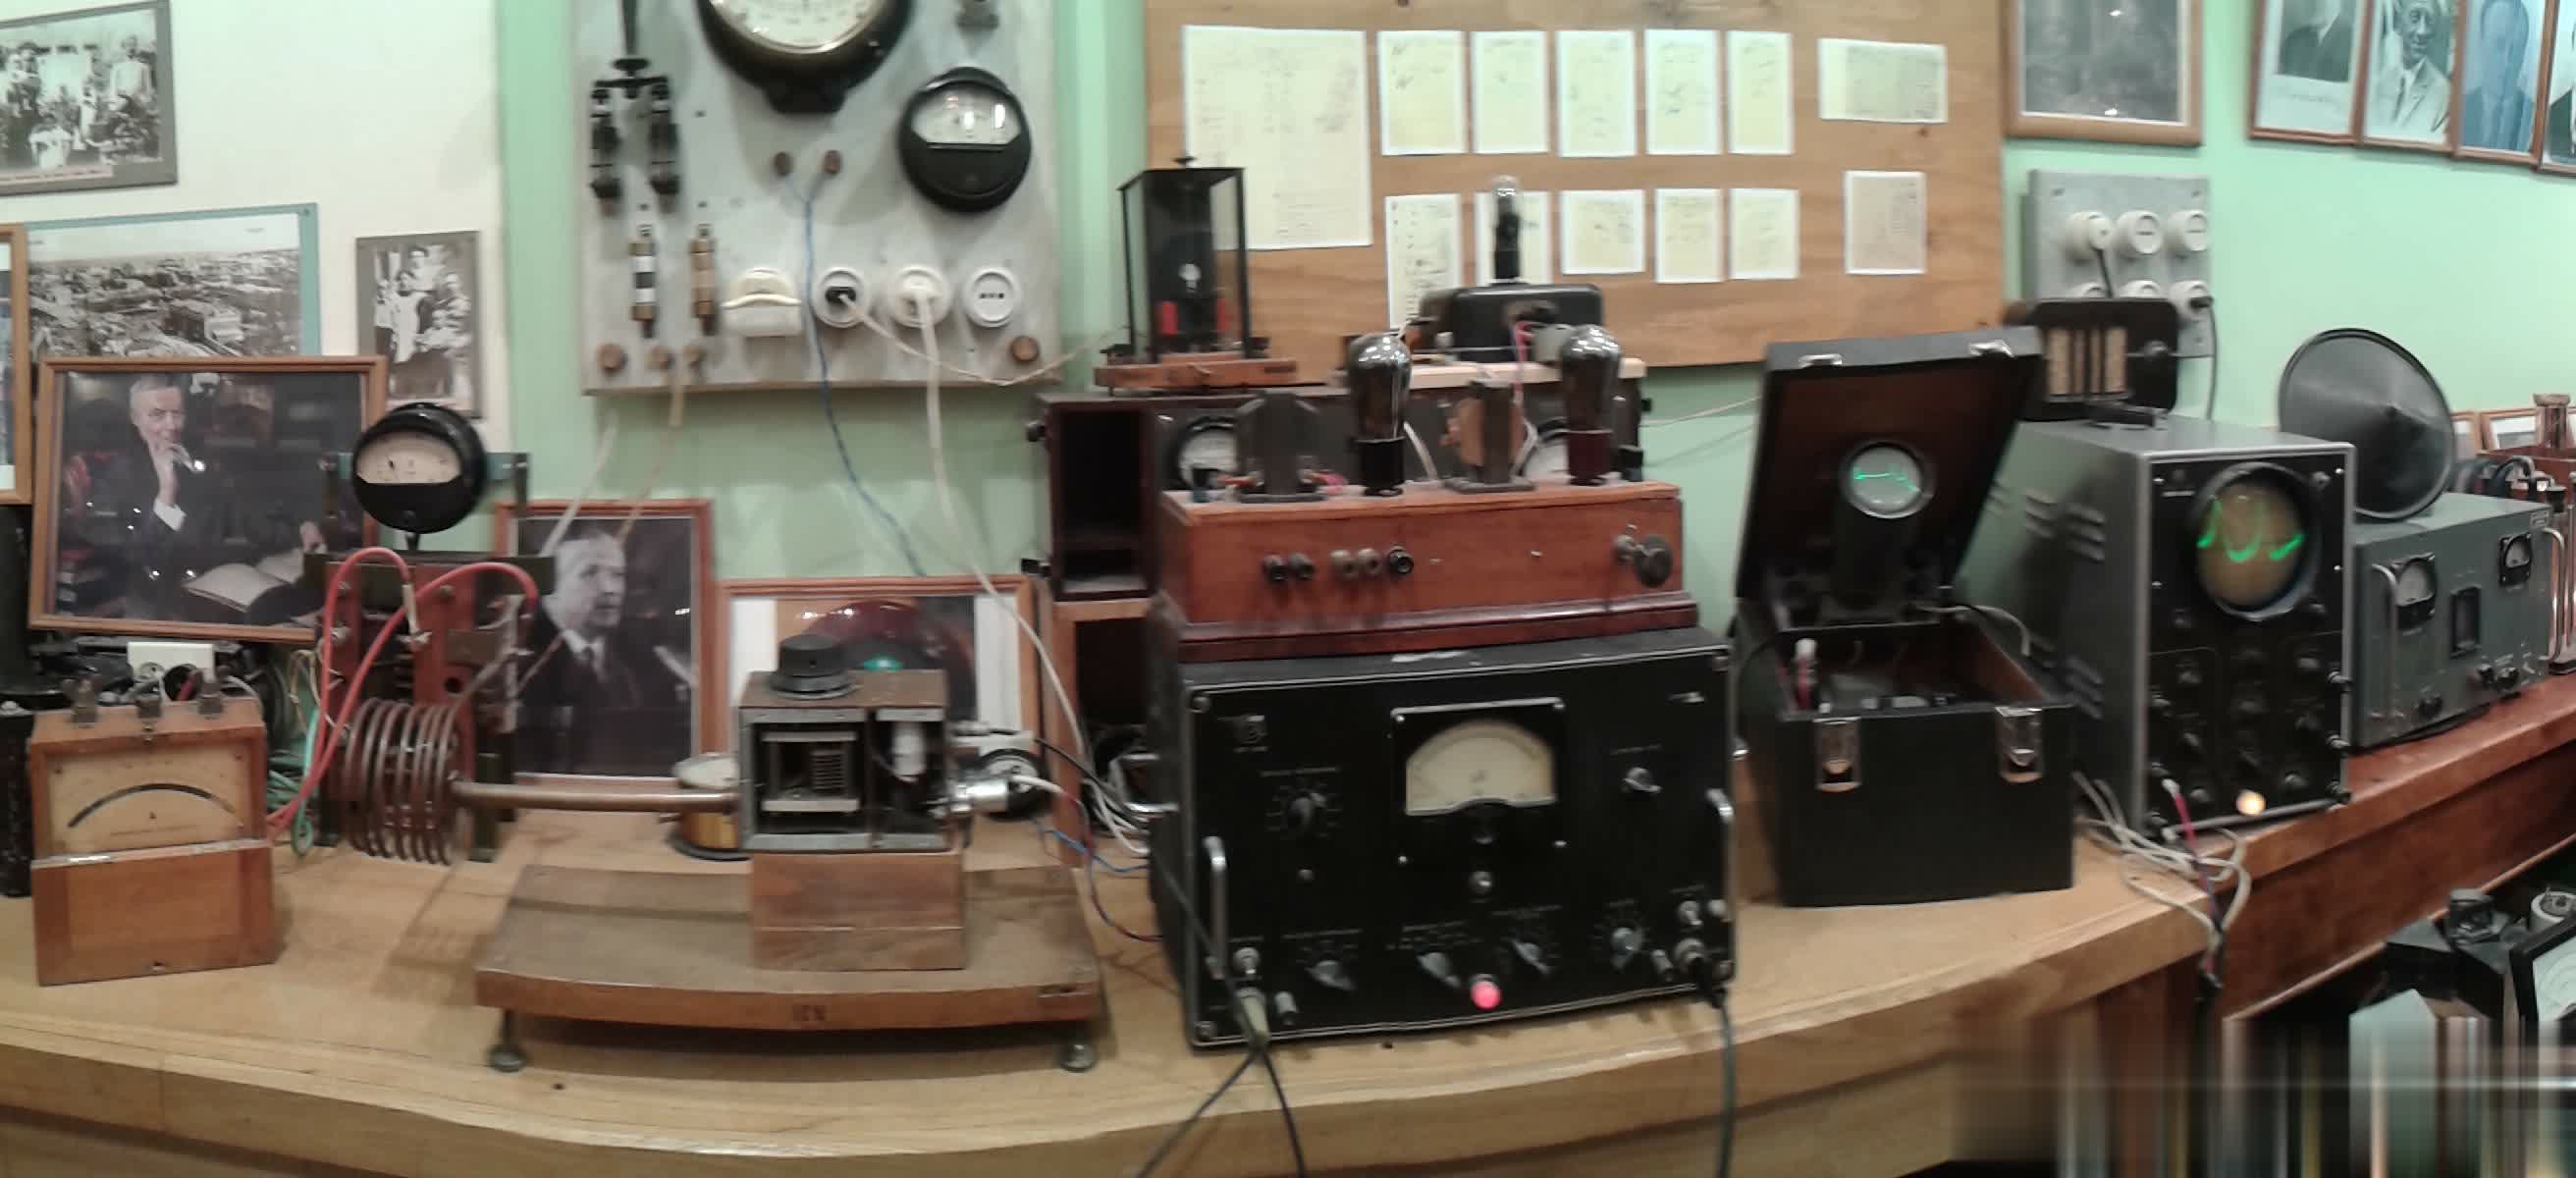
\includegraphics[scale = 0.18]{Figures/qloFRlMIUU-compress.jpg}
        \caption{Panoramic view of the reconstruction of Zavoisky's experimental setup. The signal is read out on the oscilloscope. It is preserved at the  Evgeny Zavoisky museum in the Kazan Federal University \footnote{Courtsey of the \href{http://chiralqubit.eu/a-visit-to-the-Zavoisky-museum}{CHIRALQUBIT Project}.}.}
        \label{fig:zavoisky}
    \end{figure*}
    \par
    Applications of electron magnetic spin resonance in solid state physics are of great importance. It is a very sensitive technique and has been applied in many fields. The chief of these are paramagnetic ions in crystals, unpaired electron in semi-conductors and organic free radicals, colour centres, and radiation damage centres, ferro and anti-ferro magnetic materials.


\section{Theory}
    It is well known that an electron carries a spin angular momentum, which gives it a magnetic property known as a magnetic moment. There are many materials that contains unpaired electrons. When an external magnetic field is applied, the unpaired electrons can either orient in a direction parallel or anti-parallel to the direction of the magnetic field. This creates two distinct energy levels for the unpaired electrons an measurements are taken as they are driven between the two levels. The theoretical treatment of this experiment is divided into subsections, as we build upon the physics needed to understand and perform this experiment.
    \subsection{Larmor Precession}
    Before going into the details of magnetic resonance, we need to understand what is \textit{precession}. Precession is a change in the orientation of the rotational axis of a rotating body. More specifically, the precession of the magnetic moment of an object about an external magnetic field is referred to as \textit{Larmor precession}.
    \par
    When a magnetic moment $\Vec{\mu}$ is placed in a magnetic field $\Vec{B}$, it experiences a torque which can be expressed as
    \begin{equation}
        \Vec{\tau} = \Vec{\mu} \times \Vec{B}
    \end{equation}
    \begin{figure}
        \centering
        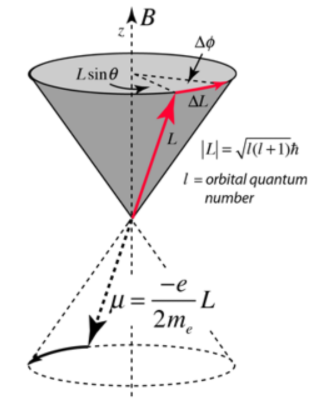
\includegraphics[scale = 0.8]{Figures/larmor.png}
        \caption{Larmor precession}
        \label{fig:larmor}
    \end{figure}
    From figure (\ref{fig:larmor}), we can write
    \begin{equation}
        \tau = \dfrac{\Delta L}{\Delta t} = \dfrac{L \sin \theta \Delta \phi}{\Delta t} = \abs{\mu B \sin \theta} = \dfrac{e}{2 m_e} LB \sin \theta
    \end{equation}
    The precession angular velocity called as Larmor frequency is
    \begin{equation}
        \omega_{Larmor} = \dfrac{d \phi}{d t} = \dfrac{e}{2 m_e} B
    \end{equation}
    In general, we can write
    \begin{equation}
        \omega = \gamma B = \dfrac{e g_e}{2 m_e} B
    \end{equation}
    where $\gamma$ is the gyromagnetic ratio ( the ratio of its magnetic moment to its angular momentum) and $g_e$ is the electron's Land\'e $g$-factor (a dimensionless quantity defined for an electron with both spin and orbital angular momenta).
    \subsection{Elementary Magnetic Resonance}
    Suppose a particle having a magnetic moment $\Vec{\mu}$ is placed in a uniform magnetic field of intensity $\Vec{H_0}$ (figure (\ref{fig:precession})). Then the moment $\Vec{\mu}$ will precess around $\Vec{H_0}$ with an angular Larmor frequency
    \begin{equation}
        \omega_0 = g_e \Bigg( \dfrac{e}{2 m c} \Bigg) H_0
    \end{equation}
    \begin{figure*}
        \centering
        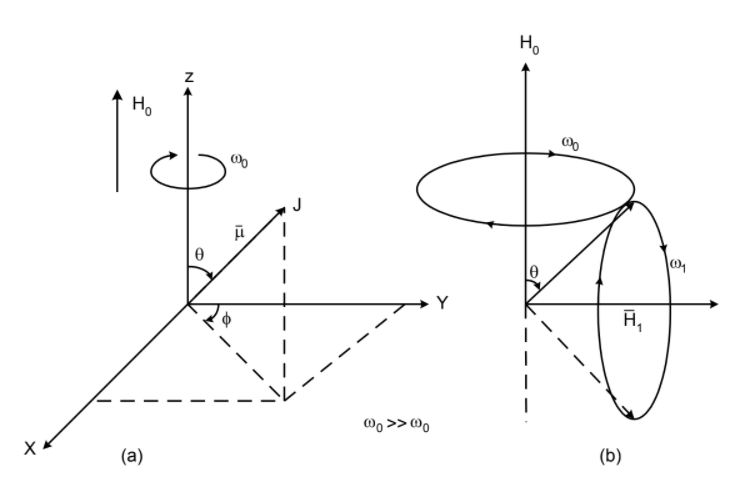
\includegraphics[scale = 0.9]{Figures/precession.png}
        \caption{Precession of a magnetic moment $\Vec{\mu}$ when placed in a magnetic field $\Vec{H_0}$. \\ (a) The spin precesses with angular frequency $\omega_0 = \gamma H_0$; the angle $\theta$ is a constant of the motion. \\ (b)  In addition to $\Vec{H_0}$ a week magnetic field $\Vec{H_1}$ is now also applied. $\Vec{H_1}$ is rotating about the $z$-axis with angular frequency $\omega_0$ and therefore $\Vec{\mu}$ precesses about $\Vec{H_1}$ with angular frequency $\omega_1 = \gamma H_1$; $\theta$ is not conserved anymore.} 
        \label{fig:precession}
    \end{figure*}
    Note that the Larmor frequency will change with the change in field strength. As seen in figure (\ref{fig:precession} (b)), an additional weak magnetic field  is introduced oriented in $xy$-plane and rotating about the $z$-axis (in the same direction as the \textit{Larmor precessing}) with an angular frequency $\omega_1$. If the frequency $\omega_1$ is different from $\omega_0$, the angle between the field $\Vec{H_1}$ and $\Vec{H_0}$ will continuously change so that their interaction will average out to zero. However, if however, $\omega_1 = \omega_0$, the angle between $\Vec{H_1}$ and $\Vec{H_0}$ is maintained and net interaction is effective. This corresponds to change in the potential energy of the particle in the magnetic field. This is the classical analogy to a transition between sub-levels with different $m$.
    \par
    Suppose that the intrinsic angular momentum of the electron $\Vec{S}$ couples with the orbital angular momentum of electron $\Vec{L}$ to give a resultant $\Vec{J}$. We know, that there are $J+1$ magnetic sub-levels labelled by the magnetic field $\Vec{H_0}$ by equal energy difference $\Delta E = g_e \mu_B H_0$ between adjacent sub-levels, where $\mu_B$ is the Bohr magneton. The quantum mechanical value of $g_e$ is given as
    \begin{equation}
    \label{eqlande}
        g_e = 1 + \dfrac{J (J+1) + S (S+1) - L (L+1)}{2 J (J+1)}
    \end{equation}
    Now, if the particle is subjected to a perturbation by an alternating magnetic field with a frequency $\nu_1$ such that the quantum $h \nu_1$ is exactly the same as the difference between the levels, $\Delta E$ and if the direction of the alternating field is perpendicular to the direction of the static magnetic field, then there will be induced transitions between neighbouring sub-levels according to the selection rules $\Delta m = \pm 1$ for magnetic dipolar radiation. Therefore, the condition for resonance is
    \begin{equation}
    \label{eqDelE}
        \Delta E = g_e \mu_B H_0 = h \nu_0 = h \nu_1
    \end{equation}
    where $\nu_1$ is the resonance frequency in cycles/sec. This requirement is identical with the classical condition $\omega_1 = \omega_0$.
    \par
    In atomic spectroscopy, we do not observe the transitions between sub-levels with different $m$ (labelled $a_1$, $a_2$, $a_3$ and selection rules $\Delta L = \pm 1$. Instead the splitting of a level is observed through small change in frequency of the radiation emitted in the transition between widely distant levels (figure (\ref{fig:energylevels})). It is clear that, if we could directly measure the frequency corresponding to a transition between the sub-levels of the same state, a much more precise knowledge of the energy splitting would be obtained.
    \begin{figure*}
        \centering
        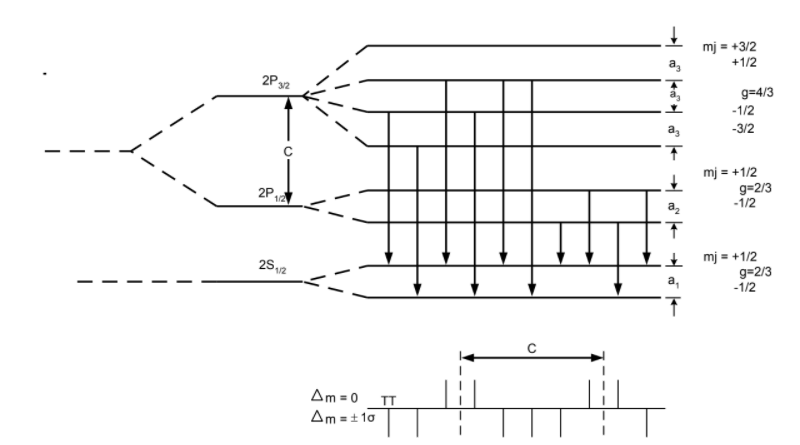
\includegraphics[scale = 1]{Figures/energylevels.png}
        \caption{Energy levels of a single valence electron atom showing a $P$ state and an $S$ state. Due to the fine structure, the $P$ state is split into a doublet with $j=2/3$ and $j = 1/2$. Further, under the influence of an external magnetic field each of the three levels is split into sub-levels as shown in the figure where account has been taken of the magnetic moment of the electron. The magnetic quantum number mi for each sub-level is also shown as is the $g$-factor for each level. The arrows indicate the allowed transitions between the initial and final states, and the structure of the line is shown in the lower part of the figure.}
        \label{fig:energylevels}
    \end{figure*}
    \par
    In this experiment we will apply the external magnetic field $\Vec{H_0}$ using a Helmholtz coil and the small magnetic field $\Vec{H_1}$ using a microwave source.



    \subsection{Origin of an ESR signal}
    Every electron has a magnetic moment and spin quantum number, $s = \dfrac{1}{2}$, with magnetic components $m_s = + \dfrac{1}{2}$ or $m_s = - \dfrac{1}{2}$. In the presence of an external magnetic field with strength $B_0$ , the electron's magnetic moment aligns itself either anti-parallel ($m_s = - \dfrac{1}{2}$) or parallel ($m_s = + \dfrac{1}{2}$) to the field, each alignment having a specific energy due to the Zeeman effect\footnote{The effect of splitting of a spectral line into several components in the presence of a static magnetic field. It is named after the Dutch physicist Pieter Zeeman, who discovered it in 1896. It is analogous to the Stark effect, the splitting of a spectral line into several components in the presence of an electric field.}:
    \begin{equation}
        E = m_s g_e \mu_B B_0
    \end{equation}
    where $g_e = 2.0023$ for the free electron. Therefore, the separation between the lower and the upper state is $\Delta E = g_e \mu_B B_0$ for unpaired free electrons. This equation implies (since both $g_e$ and $\mu_B$ are constant) that the splitting of the energy levels is directly proportional to the magnetic field's strength (see figure (\ref{fig:ESRsplit})).
    \begin{figure}
        \centering
        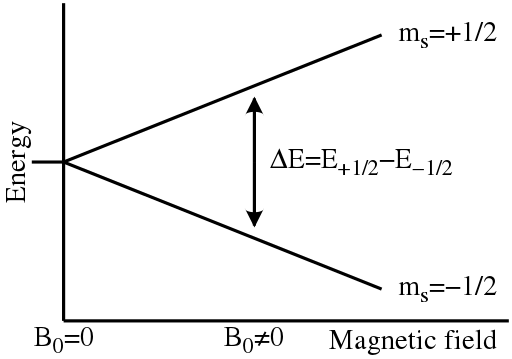
\includegraphics[scale = 0.4]{Figures/EPR_splitting.svg.png}
        \caption{The splitting of the energy levels is directly proportional to the magnetic field's strength}
        \label{fig:ESRsplit}
    \end{figure}
    An unpaired electron can change its electron spin by either absorbing or emitting a photon of energy $h \nu$ such that the resonance condition, $h \nu = \Delta E$ is obeyed. This leads to the fundamental equation of ESR spectroscopy:
    \begin{equation}
        h \nu = g_e \mu_B B_0
    \end{equation}
    By increasing an external magnetic field, the gap between the $m_s = + \dfrac{1}{2}$ and $m_s = - \dfrac{1}{2}$ energy states is widened until it matches the energy of the microwaves, as represented by the double arrow in the diagram above. At this point the unpaired electrons can move between their two spin states. Since there typically are more electrons in the lower state, due to the Maxwell–Boltzmann distribution, there is a net absorption of energy, and it is this absorption that is monitored and converted into a spectrum. The upper spectrum below is the simulated absorption for a system of free electrons in a varying magnetic field. The lower spectrum is the first derivative of the absorption spectrum. The latter is the most common way to record and publish continuous wave ESR spectra.
    \begin{figure}
        \centering
        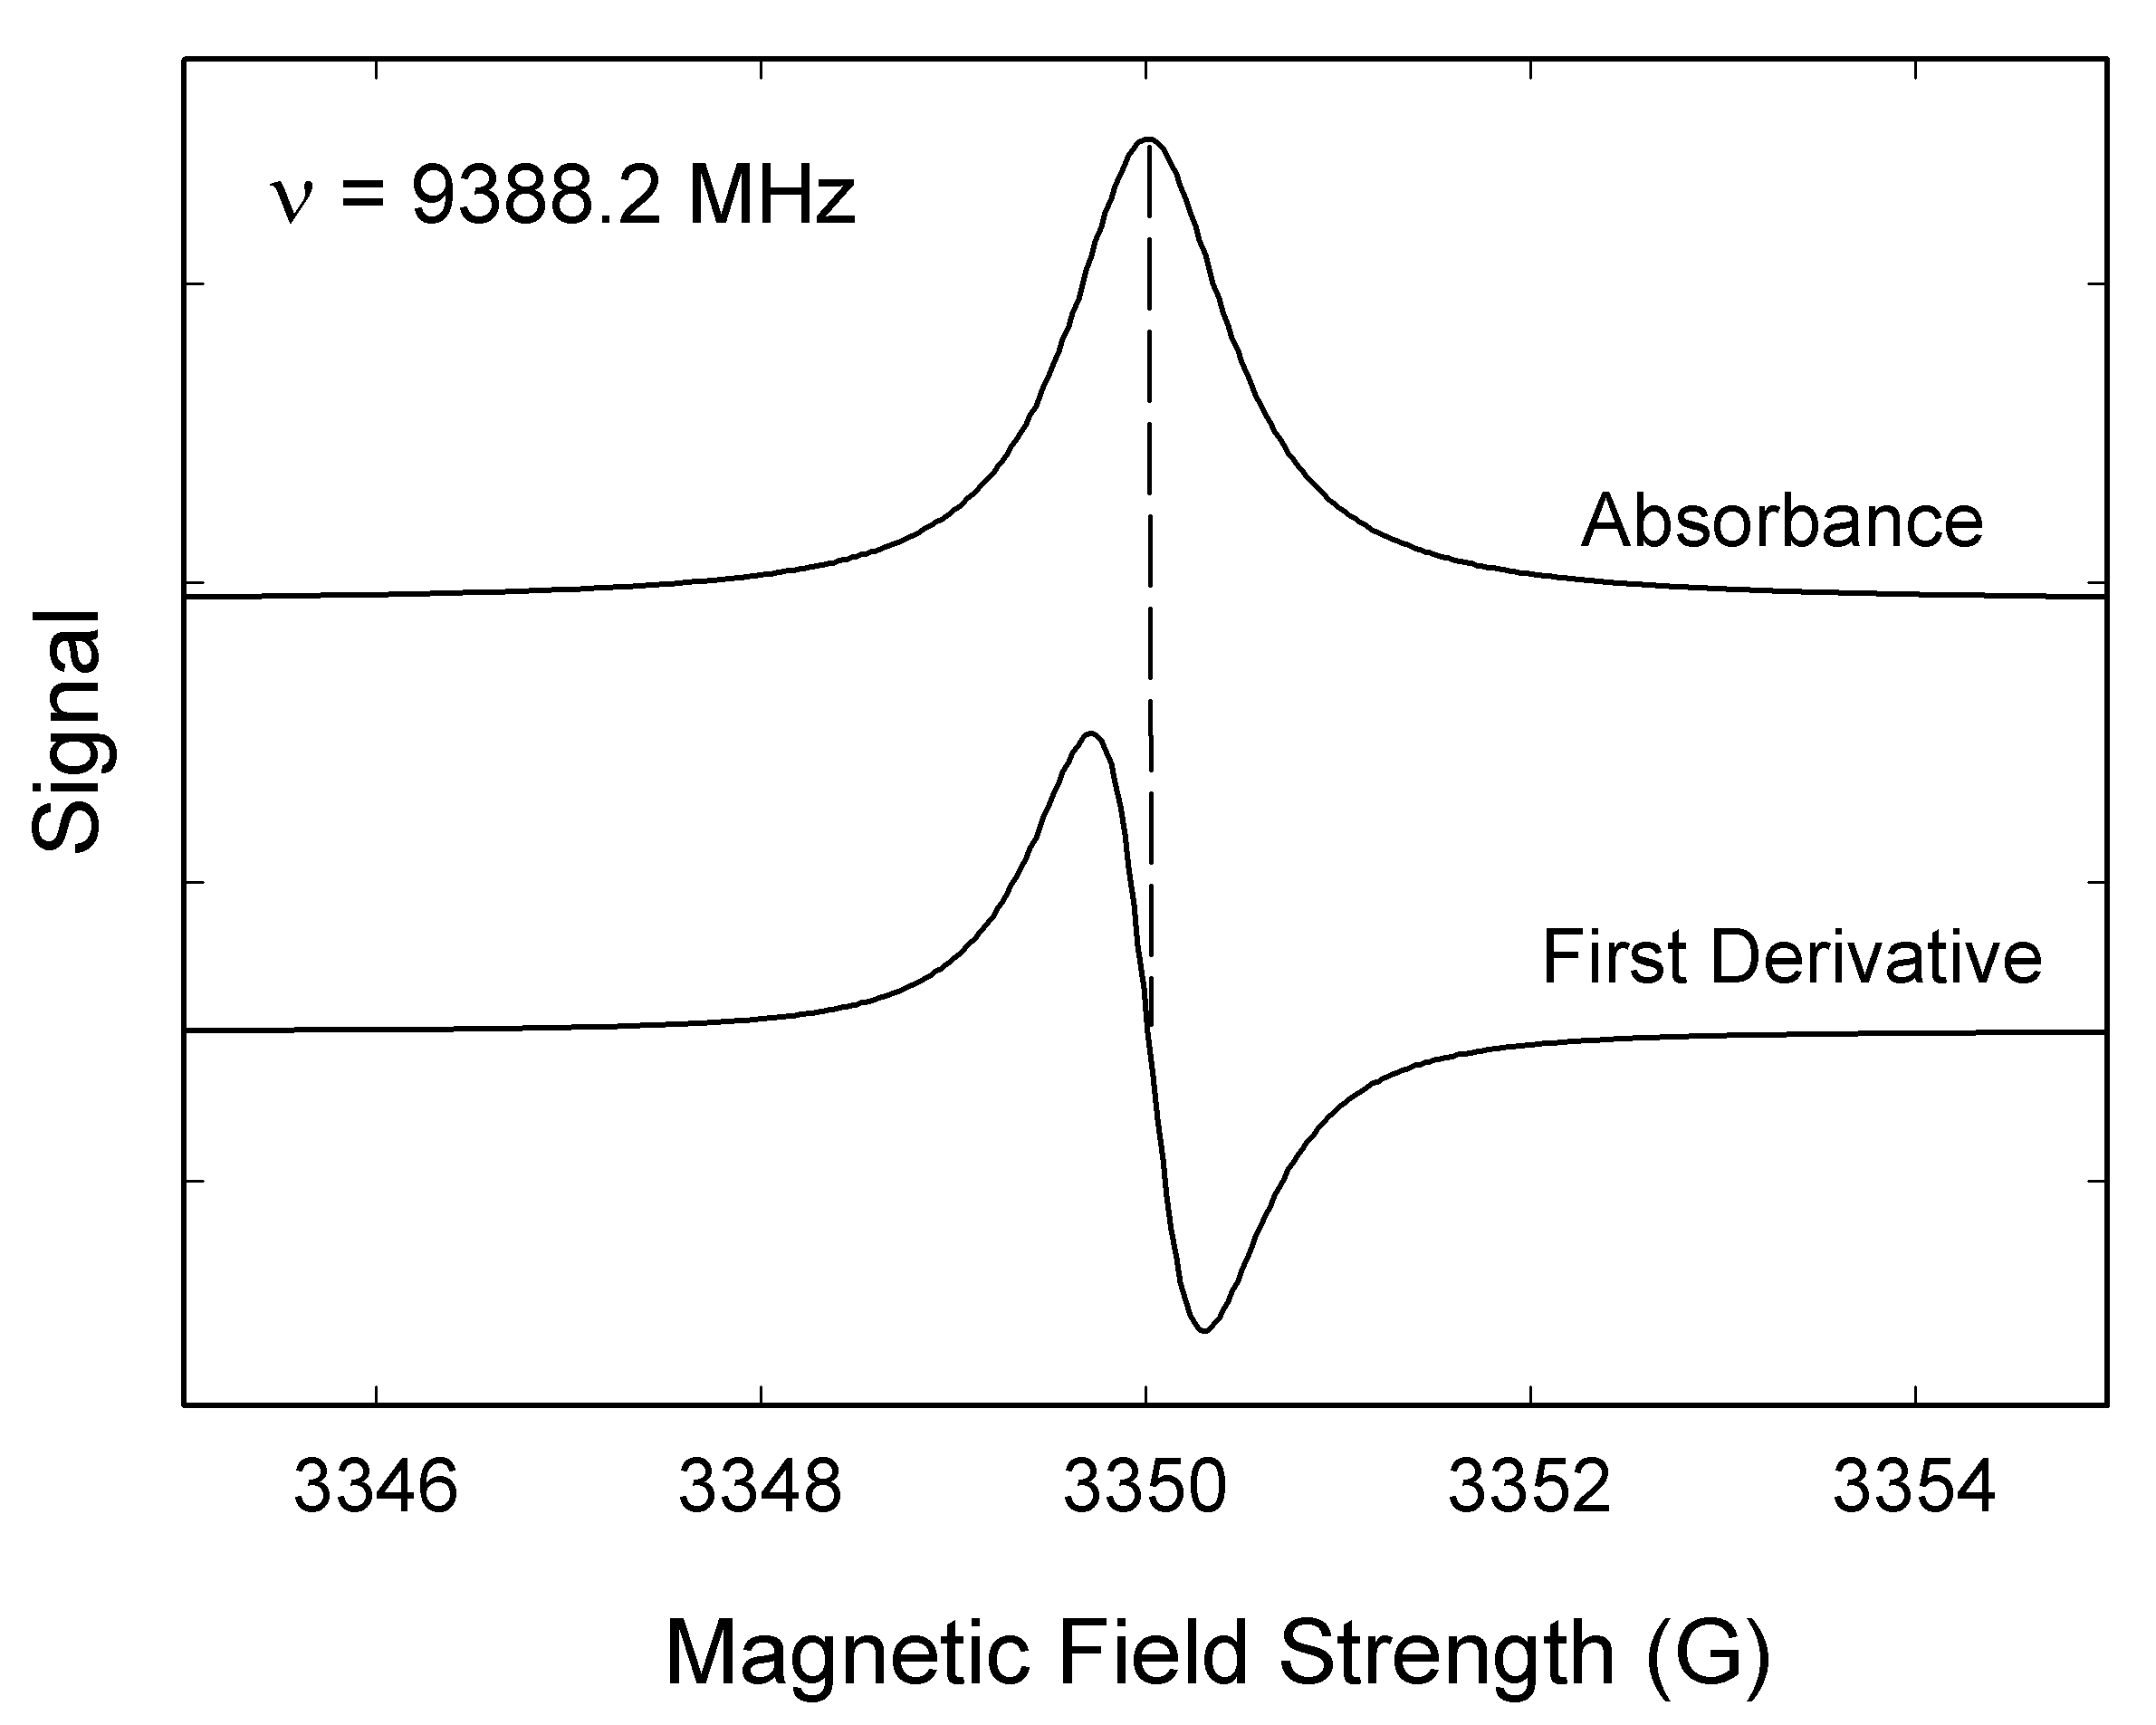
\includegraphics[scale = 0.1]{Figures/EPR_lines.png}
        \caption{The shape of ESR signal against the applied magnetic field strength for microwave frequency $\SI{9388.2}{\mega \hertz}$}
        \label{fig:ESRline}
    \end{figure}
    For example, for the microwave frequency of $\SI{9388.2}{\mega \hertz}$, the predicted resonance occurs at a magnetic field of about $B_0 = h \nu / g_e \mu_B = \SI{0.3350}{\tesla} = \SI{3350}{\gauss}$ (see figure (\ref{fig:ESRline})).
    \par
    The ESR spectrum is usually directly measured as the first derivative of the absorption. This is accomplished by using field modulation. A small additional oscillating magnetic field is applied to the external magnetic field at a typical frequency of $\SI{100}{\kilo \hertz}$ (see figure (\ref{fig:ESRfm})).
    \begin{figure}
        \centering
        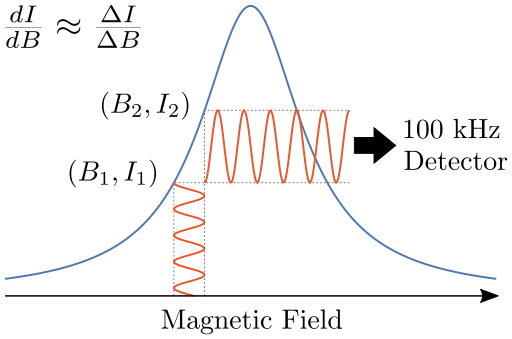
\includegraphics[scale = 0.4]{Figures/EPR_Field_Modulation.svg.png}
        \caption{The field oscillates between $B_1$ and $B_2$ due to the superimposed modulation field at $\SI{100}{\kilo \hertz}$. This causes the absorption intensity to oscillate between $I_1$ and $I_2$. The larger the difference the larger the intensity detected by the detector tuned to $\SI{100}{\kilo \hertz}$ (note this can be negative or even 0). As the difference between the two intensities is detected the first derivative of the absorption is detected.}
        \label{fig:ESRfm}
    \end{figure}
    
    
    \subsection{ESR in Macroscopic systems}
    Now that we have understood magnetic resonance at the quantum mechanical level, we can now advance to macroscopic objects like solids. The behaviour of a paramagnetic substance in a magnetic field will depend on the interaction of the particles with one another and with the diamagnetic particles. There are mainly two types of interactions: \textbf{\textit{spin-spin}} (where the spin interacts with a neighbouring spin but the total energy of the spin system remains constant) and \textbf{\textit{spin-lattice}} (where the electron spin interact with entire solid or liquid, transforming energy from the spin system to the lattice which act as a thermal reservoir). As a matter of fact it is the spin-lattice interaction that makes possible the observation of energy absorption from the radio-frequency field when the resonance frequency is reached.
    \par
    To understand this last statement, consider a paramagnetic substance in a magnetic field $\Vec{H_0}$ and say the equilibrium state has been reached. The population of individual energy levels will be determined by the Boltzmann distribution $e^{-g_e \mu_0 H_0 m/ kT}$ where $m$ is the magnetic quantum number. It can be seen that the population of the lower energy levels are greater than those of the upper levels and, therefore when a periodic magnetic field with a resonance frequency is switched on; the number of induced radiation events will be more and as a result the substance will absorb energy from the radio-frequency field. Thus, two opposing processes take place in ESR. The radio frequency field tends to equalise the population of various levels and the spin lattice interaction tends to restore the Boltzmann distribution by conversion of the energy absorbed from the radio-frequency field into heat.
    \par
    The the mechanism through which the electron return from an excited state to the ground state or relax back to the ground state is known as \textit{relaxation} in the field of magnetic resonances  and the time taken by the process is called the \textit{relaxation time}. This complete process may be considered as two state process (provided the spin-spin interactions are much stronger than the spin-lattice interaction). First, the energy is absorbed from the radio frequency magnetic field and the equilibrium is established inside the `spin system'. The time taken by this process is known as the \textit{spin-spin relaxation time} and is a measure of the rate at which magnetic energy can be distributed within the spin system though total energy is conserved. Secondly, an exchange of energy occurs between the spin system and the lattice. The time taken is known as the \textit{spin-lattice relaxation time} and is a measure of the rate of transfer of energy from the spin system to the lattice.
    \par
    In optical spectroscopy of the relaxation time is usually very short ($\SI{e-8}{\second}$) so that the relaxation time does not impede the absorption rate. In radio frequency, on the other hand, typical relaxation times are in milliseconds or longer and the spin do not have time to relax if the energy is supplied at a faster rate. This situation is called the \textbf{saturation state}. In other words, no additional energy is absorbed, if the radio-frequency field power is increased beyond certain level.
    \par
    The effect of the spin-spin interaction is to slightly shift the exact position of energy level of any individual spin in the external field. This energy shift clearly depend on the relative orientation and distance of the spin and thus is different for each spin, resulting in apparent broadening of the energy level. Another way of thinking of the spin-spin interaction is that one electron spin produce a local magnetic field at the position of another spin. Thus, the width of absorption line due to spin-spin interaction may be estimated as $\dfrac{1}{T'}$, where $T'$ is the spin-spin relaxation time.
    \par
    If the spin-lattice interactions are not weak the spin lattice relaxation time $T$ will also be introduced. Let us consider the probability of a transition of an individual paramagnetic particle from one magnetic level to another under the influence of thermal motion. If the probability per second is equal to $A$, $T \sim \dfrac{1}{A}$ and the absorption line width would be of the order of $\dfrac{1}{T}$. In general case, however, the absorption line width may be estimated as $\dfrac{1}{T} + \dfrac{1}{T'}$.
    \par
    Thus, we see that from the width of absorption line it is possible to measure the relaxation time. In fact most of the research in this field involve the study of relaxation phenomena which in turn provide information about internal interactions in solids and liquids. The position and number of lines of paramagnetic resonance absorption also depend on the internal interactions.
    
    
\section{Formulation}
    Now that we have gone through the theory, we can formulate the physics which will aid us in calculating the different parameters in the experiment.
    \par
    If an electron of mass $m$ and charge $e$ is located in an electromagnetic field with vector potential $\Vec{A}$ and scalar potential $\phi$, then its steady-state energy level and characteristic states are given by the solutions of the Dirac equation.
    \par
    If the equation is solved for the c, component of the state spinor\footnote{an element of a complex vector space that can be associated with Euclidean space}, it reads:
    \begin{equation}
    \label{eqpi2}
        \Big( \Vec{\pi^{2}} + \mu_B 2 \Vec{S} \cdot \Vec{B} \Big) \pi_1 = \epsilon \psi_1
    \end{equation}
    where the Bohr magneton, $\mu_B = \dfrac{eh}{2 m_e c} = \SI{9.27e-27}{\ampere \metre \squared}$ and $\Vec{\pi} = \Vec{p} + \dfrac{e}{c} \Vec{A}$, $\Vec{p}$ being the momentum, $c$ being the velocity of light, $h = \SI{6.626e-34}{\joule \second}$ is the Planck's constant, $\Vec{S}$ is the electron spin operator and $\Vec{B} = \Rot \Vec{A}$. Finally, $\epsilon = \dfrac{1}{2} \Big( 1 + (E/mc)^2 \Big) \Big( E - mc^2\Big)$ is approximately the excess of energy over the residual mass energy.
    \par
    For a free electron in a uniform magnetic field, the second term (Zeeman term) interchanges with the first in the Hamiltonian operator of (\ref{eqpi2}), and the energy level
    \begin{equation}
        \epsilon = \epsilon_0 + \mu_B 2 S_Z B_Z
    \end{equation}
    is obtained if the $z$-axis lies in the direction of the magnetic field. $\epsilon_0$ is the energy of the electron without a magnetic field. If the diamagnetic contribution from the first term of (\ref{eqpi2}) is disregarded in the general case, then for the electron in a uniform magnetic field, the interaction Hamiltonian operator with the magnetic filed, (Zeeman effect) is
    \begin{equation}
        H_Z = \mu_B \Vec{B} \cdot (\Vec{L} + 2 \Vec{S})
    \end{equation}
    where $\Vec{L}$ and $\Vec{S}$ are the operators of the orbital and spin angular momentum respectively. In addition, the spin-orbit interaction
    \begin{equation}
        H_{so} = \lambda \cdot \Vec{S} \cdot \Vec{L} 
    \end{equation}
    should be taken into account, so that only the total angular momentum
    \begin{equation}
        \Vec{J} = \Vec{L} + \Vec{S}
    \end{equation}
    is a conserved value.
    \par
    In this case, $H_Z$ can be written as
    \begin{equation}
    \label{eqHz}
        H_Z = \mu_B g_e \Vec{B} \cdot \Vec{J}
    \end{equation}
    where $g_e$ is the $g$-factor given by (\ref{eqlande}). Disregarding the influence of the nuclear spin, the energy levels of $H_Z$, for magnetic fields in the $z$-direction, are
    \begin{equation}
        E_Z = \mu_B g_e B m_j
    \end{equation}
    with $m_j = j, j-1, \ldots -j$. The selection rule for magnetic transitions of the electron spin resonance experiment is
    \begin{equation}
        \Delta m_j = \pm 1
    \end{equation}
    so that the absorption condition reads
    \begin{equation}
        \mu_B g_e B = \Delta E = h \nu
    \end{equation}
    In many cases, especially with molecular radicals, the angular momentum $L$ of the unpaired electron is extinguished by the electric fields of the neighbouring atoms and molecules. In the case of DPPH (the paramagnetic sample used in the experiment), $L = 0$ and therefore
    \begin{equation}
        g_e = 2
    \end{equation}
    In (\ref{eqHz})
    \begin{equation}
        \Vec{\mu} = \mu_B \cdot g_e \cdot \Vec{J}
    \end{equation}
    is the magnetic moment of an electron with the angular momentum $\Vec{J}$ in units of the Bohr magneton $\mu_B$.
    \par
    If account is also taken of the exchange of virtual photons between the electron and a radiation field in the static limit through inclusion of the vertex corrections in increasing order, a modified abnormal magnetic moment of the electron is obtained as a series in the fine-structure constant $\alpha$:
    \begin{equation}
    \label{eqalpha}
        \begin{split}
            \alpha
            &= \dfrac{e^2}{hc} \\
            \Vec{\mu}
            &= \mu_B \Big( 1 + \dfrac{\alpha}{2 \pi} - 0.328 \dfrac{\alpha^2}{\pi^2} + \ldots \Big) g_e \Vec{J}
        \end{split}
    \end{equation}
    The correction factor in the parentheses of equation (\ref{eqalpha}) is generally taken into account in $g_e$, so that then $g_e \neq 2$.
    \par
    By supplying the corresponding energy, transitions can be induced between the levels:
    \begin{equation}
    \label{eqge}
        h \nu = g_e \mu B H
    \end{equation}
    The probability of transition depends on the occupation number and on the transition matrix elements. The latter are the same for absorption and emission processes.
    \par
    Because of the interactions of the spins with the lattice or with one another, the levels are not sharply defined, and this leads to a line width of the absorption spectrum and prevents an equipartition of the levels (saturation) because of the corresponding relaxation processes. The occupation numbers are given in accordance with the Boltzmann relation by:
    \begin{equation}
        \dfrac{N_2}{N_1} = e^{- \frac{\Delta E}{kT}} = e^{- \frac{g_e \mu_B B}{kT}}
    \end{equation}
    where $k$ is the Boltzmann constant.
    \begin{figure*}
        \centering
        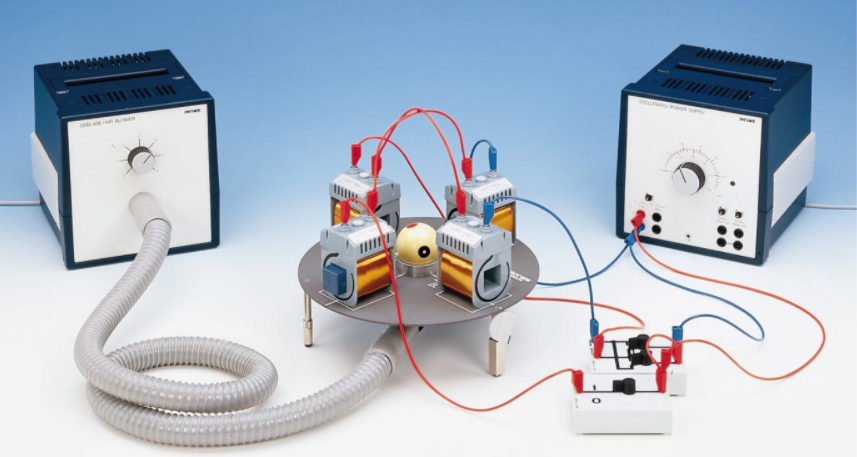
\includegraphics[scale = 0.9]{Figures/esrmodelexpt.png}
        \caption{ESR model experiment}
        \label{fig:my_label}
    \end{figure*}
    
    
\section{\label{sec:setup}Description of the Setup}
    \begin{figure}
        \centering
        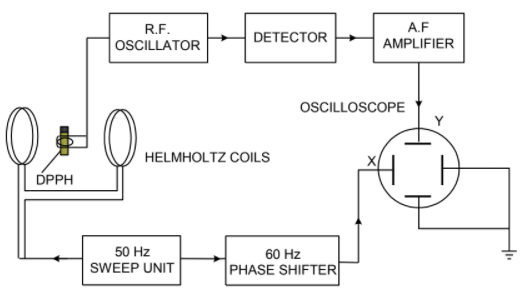
\includegraphics[scale = 0.75]{Figures/blockdgESR.png}
        \caption{ Block Diagram of the ESR Set}
        \label{fig:block}
    \end{figure}
    \begin{figure*}
        \centering
        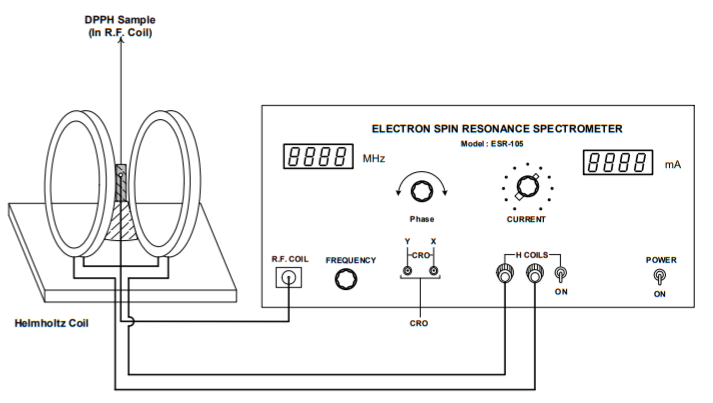
\includegraphics[scale = 1]{Figures/paneldgESR.png}
        \caption{Panel Diagram of Electron Spin Resonance Spectrometer, ESR-105}
        \label{fig:panel}
    \end{figure*}
    \begin{figure}
        \centering
        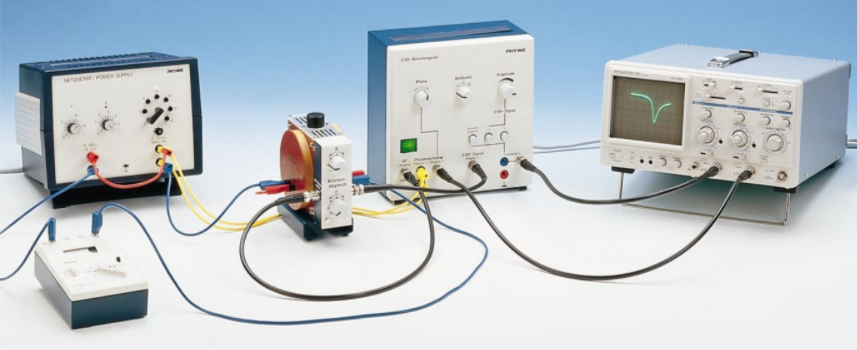
\includegraphics[scale = 0.4]{Figures/setupcharactcurves.png}
        \caption{Experimental set-up for determining characteristic curves.}
        \label{fig:characurves}
    \end{figure}
    A block diagram of the ESR Spectrometer is given in figure (\ref{fig:block}) and panel diagram is given in the figure (\ref{fig:panel}). The experimental set-up for determining the characteristic curves is given in figure (\ref{fig:characurves}). The various components of the ESR spectrometer are detailed as follows:
    \begin{enumerate}
        \item \textbf{Basic circuit}: The first stage of the ESR circuit consists of a critically adjusted (marginal) radio frequency oscillator having a frequency range of approximately $\SI{12}{\mega \hertz}$ to $\SI{16}{\mega \hertz}$. A marginal oscillator is required here so that the slightest increase in its load decreases the amplitude of oscillation to an appreciable extent. The sample is kept inside the tank coil of this oscillator, which in turn, is placed in the 50Hz magnetic field, generated by the Helmholtz coils. At resonance, i.e. when the frequency of oscillation equal to the Larmor's frequency of the sample, the oscillator amplitude registers a dip due to the absorption of power by the sample. This obviously, occurs periodically - four times in each complete cycle of the Helmholtz coils supply voltage. The result is in amplitude modulated carrier (figures (\ref{fig:4AatA}) and (\ref{fig:4AatB})) which is then detected using a diode detector and amplified by a chain of three low noise, high gain audio - frequency amplifiers of excellent stability. A sensitivity control is provided in the amplifier to suit the input requirement of any oscilloscope.
        \begin{figure}
            \centering
            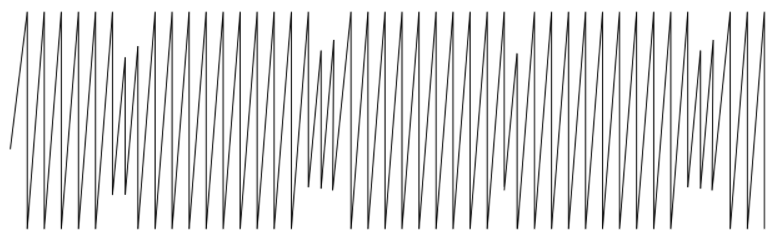
\includegraphics[scale = 0.5]{Figures/fig4AatA.png}
            \caption{The amplitude modulated carrier at $A$ from the circuit diagram in figure (\ref{fig:4B1})}
            \label{fig:4AatA}
        \end{figure}
        \begin{figure}
            \centering
            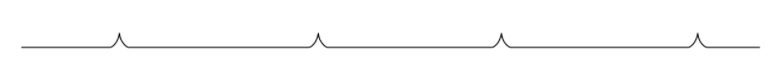
\includegraphics[scale = 0.5]{Figures/fig4AatB.png}
            \caption{The amplitude modulated carrier at $B$ from the circuit diagram in figure (\ref{fig:4B1})}
            \label{fig:4AatB}
        \end{figure}
        \item \textbf{Phase shifter}: In order to make it possible to use an ordinary displaying type oscilloscope, instead of a measuring oscilloscope which preserve the phase between X and Y plates signals, a phase shifter is provided. This can compensate the phase difference which is introduced in the amplification stage of the ordinary oscilloscope.
        \par
        The circuit diagram of the phase shifter is shown in figures (\ref{fig:4B1}). The primary of the transformer is fed from the $\SI{220}{\volt}$, $\SI{50}{\hertz}$ (or $\SI{1100}{\volt}$, $\SI{60}{\hertz}$) mains and the secondary is centre tapped developing $V_1 - 0 - V_1$ (say). The operation of the circuit may be explained with the help of the vector diagram shown in figure (\ref{fig:4B2}). The vectors $OA$ and $BO$ represent the voltage developed in the secondary, in phase and magnitude. The current flowing in the circuit $ADB$ leads the voltage vector $BA$ due to the presence of capacitor $C$ and current is shown in the diagram as $I$. Voltage developed across resistance $R$, i.e. $VR$ is in phase with the current $I$, and the voltage across across capacitor $V_C$ is $90 \degree$ (lag) out of phase with the current. The vector sum of $V_C$ and $V_R$ is equal to $2 V_1$. These are also plotted in the diagram. It is clear from the diagram that as $R$ is varied, $V_R$ will change and the point $D$ will trace a semicircle, shown dotted. The vector $OD$, or the voltage across points $O$ and $D$, will, therefore, have a constant magnitude equal to $V_1$ and its phase, variable from $0 \degree$ to $180 \degree$. This is the voltage which is fed to the X-amplifier of the oscilloscope to correct for any phase change which might have taken place in the rest of the circuit.
        \begin{figure}
            \centering
            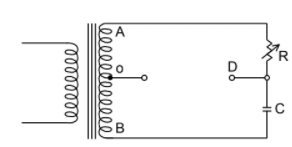
\includegraphics{Figures/fig4B1.png}
            \caption{Circuit diagram of the phase shifter circuit}
            \label{fig:4B1}
        \end{figure}
        \begin{figure}
            \centering
            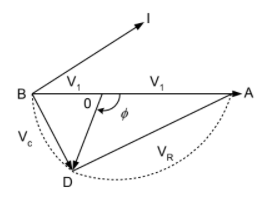
\includegraphics{Figures/fig4B2.png}
            \caption{Vector diagram of the phase shifter circuit}
            \label{fig:4B2}
        \end{figure}
        \item \textbf{50 Hertz sweep unit}: For modulation with a low frequency magnetic field, a $\SI{50}{\hertz}$ current flows through the Helmholtz coils. As the resonance in this frequency range occurs at low magnetic fields, no static $DC$ magnetic field is required.
        \item \textbf{Power supplies}:
            \begin{enumerate}
                \item \textit{$DC$ power supply}: : The ESR circuit requires a highly stabilised almost ripple free voltage. These are obtained using integrated circuit regulator.
                \item \textit{Helmholtz coils power supply}: The Helmholtz coils power supply consists of a step down transformer ($\SI{220}{\volt}$ to $\SI{35}{\volt}$ $AC$). Variable coil current is provided in 10 steps using a band switch, while the current is displayed on a $3 \frac{1}{2}$ digit panel meter. The output is taken from the two terminals provided on the panel.
            \end{enumerate}
        \item \textbf{Helmholtz coils}: There are two coils exactly alike and parallel to each other, so connected that current passes through them in the same direction. The two coils increase the uniformity of the field near the centre. There are 500 turns in each coil, the diameter of windings is $\SI{15.4}{\centi \metre}$ and the separation between the coils is $\SI{7.7}{\centi \metre}$. In the centre of the coils, an attachment is provided to keep the sample in place and to minimise shocks and vibrations.
        \item \textbf{Test sample}: A test sample, Diphenyl Picryl Hydrazyl (DPPH) (figure (\ref{fig:dpph})) is placed in a plastic tube, which itself is in the induction coils. This increases the filling factor to the maximum. DPPH is a free radical and widely used as a standard for ESR measurements.
        \begin{figure}
            \centering
            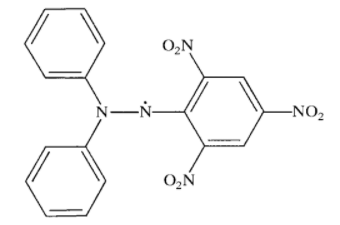
\includegraphics{Figures/dpph.png}
            \caption{Chemical structure of DPPH (2,2-Diphenyl-1-picrylhydrazyl, (free radical, 95\%))}
            \label{fig:dpph}
        \end{figure}
        \item \textbf{Control and terminals}: (refer to the panel diagram in figure (\ref{fig:panel})).
            \begin{enumerate}
                \item Mains : To switch 'ON' or 'OFF' the ESR Spectrometer.
                \item Phase : To adjust the phase between X and Y plates signals. 
                \item Current : To control current in Helmholtz coils. 
                \item 'H' Coils : Terminals and switch for Helmholtz coils. 
                \item Frequency : To adjust the frequency of the Oscillator. 
                \item X,Y,E : For X, Y and Earth terminals of the Oscilloscope.
            \end{enumerate}
        \item \textbf{Oscilloscope}: Any Oscilloscope, normally available in the laboratory of the following specifications or better, will be quite suitable for the observation of ESR resonance: a screen of diameter $\SI{12.5}{\centi \metre}$ and vertical amplifier sensitivity of $\SI{50}{\milli \volt \per \centi \metre}$.
    \end{enumerate}
     

\section{Experimental Procedure}
    A symmetrically fed bridge circuit (figure (\ref{fig:bridge})) contains a variable resistor $R$ in one branch and a high-quality tuned circuit (resonator) in the other. The specimen is located in the coil of the tuned circuit. Normally, the bridge is balanced so that the complex impedance of both branches is the same and consequently there is no voltage between points $a$ and $b$. If the external magnetic field is now so adjusted that the resonance absorption occurs in the specimen, the bridge becomes unbalanced and the voltage set up between $a$ and $b$ rectified and amplified.
    \begin{figure}
        \centering
        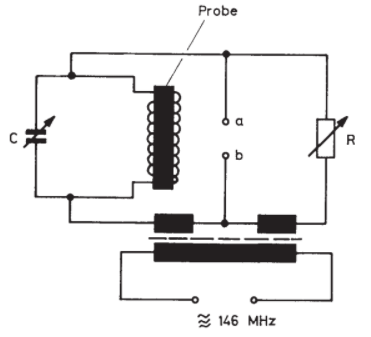
\includegraphics{Figures/measuringbridge.png}
        \caption{Measuring bridge of the ESR apparatus.}
        \label{fig:bridge}
    \end{figure}
    If the magnetic field is modulated with $\SI{50}{\hertz}$ $AC$ (voltage $\SI{2}{\volt}$), the resonance point is passed through 100 times a second (figure (\ref{fig:magfields})), and the absorption signal can be displayed on an oscilloscope, provided the x-deflection is driven with the same $AC$ voltage in the correct phase.
    \begin{figure}
        \centering
        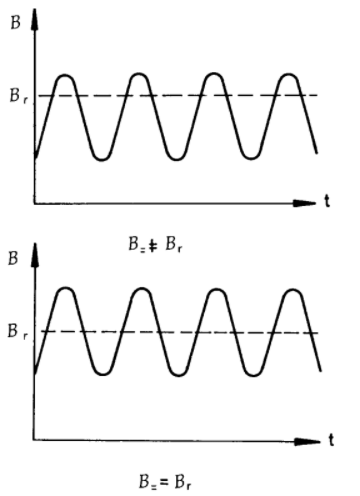
\includegraphics{Figures/magfields.png}
        \caption{The magnetic field $B$ is compounded from a $DC$ field $B_{=}$ and an alternating field $B_{\sim}$, so that $B = B_{=} + B_{\sim}$. Through $I_{=}$, $B_{=}$ is to be adjusted so that $B_{=} = B_r$}
        \label{fig:magfields}
    \end{figure}
    \par
    First, the bridge has to be balanced. In doing this (without external magnetic field),`R' on the resonator is brought to its central position and `C' to the left-hand stop. On the ESR power supply, key 8 `bridge balancing' (see operating instructions) is pressed, the oscilloscope input is switched to $DC$ and $\SI{1}{\volt \per \centi \metre}$ and the line is brought to the zero with 12 `Zero' (beforehand bring to zero with `Position' in GND setting). The wiring diagram is given in figure (\ref{fig:wiring}).
    \begin{figure}
        \centering
        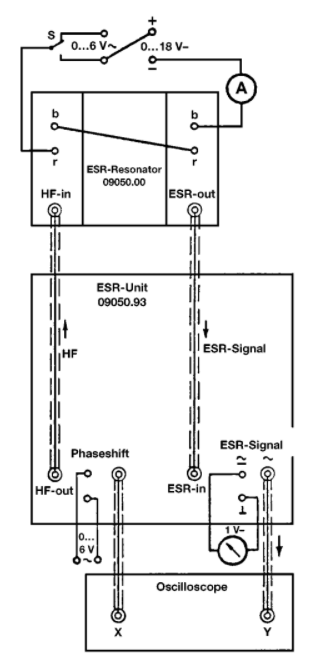
\includegraphics{Figures/wiringdg.png}
        \caption{Wiring diagram}
        \label{fig:wiring}
    \end{figure}
    \par
    The operating instructions are as follows:
    \begin{enumerate}
        \item The `H-coil power' is switched ON and the current is adjusted to $\SI{150}{\milli \ampere}$.
        \item The frequency and phase on the front panel of ESR spectrometer is set to \textit{centred}.
        \item Observe four peaks on the Screen of CRO. Now adjust the FREQUENCY of the Spectrometer and SENSITIVITY of the CRO to obtain the best results (i.e. sharp peaks and good signal to noise ratio).
        \item Adjust the PHASE knob to coincide the two peaks with the other two as far as possible.
        \item Adjust the orientation of Helmholtz coils with respect to the main unit for best overlap of base lines.
        \item To calibrate the X-plate of CRO in terms of magnetic field proceed as follows, the X amplifier (CRO) is adjusted to obtain the maximum X deflection (say 'P' divisions).
        \item Read current flowing in Helmholtz coils and calculate the magnetic field.
            \begin{equation}
            \label{eqH}
                H = \dfrac{32 \pi n}{10 \sqrt{125} \cdot a} \cdot I
            \end{equation}
        where $n$ is the number of turns in the coil, $a$ is the radius of the coils and $I$ is the current (in amp) flowing through the coils. This is the root mean square (rms) field. The peak to peak field will be $2 \sqrt{2} H$ and represents `P' division of the CRO X plate. The zero field is at the middle point.
        \item Measure the positions of the two peaks. These should be at equal distances from the middle point (say `Q' division).The magnetic field at the resonance is thus
            \begin{equation}
            \label{eqH0}
                H_0 = \dfrac{2 \sqrt{2} H}{P} \cdot Q \text{ gauss}
            \end{equation}
        \item Increase the horizontal sensitivity of the Oscilloscope to the maximum within the linear range.
        \item Obtain the best possible resonance peaks by varying the frequency, detection level and vertical sensitivity of the oscilloscope, keeping the current at 150 mA (say). 
        \item Keep the frequency fixed but vary the current flowing through the coils and measure the corresponding horizontal separation between the two peaks (2Q) after adjusting the phase. Take five to six sets of observations.
        \item Draw a graph in 1/I Vs Q which should be a straight line. Calculate the g-factor using the QI value from the graph.
        \item Repeat the experiment with different frequency. 


    \end{enumerate}
    
    
\section{Observations}
    The make of the instrument is SES Instruments, Roorkee. The preliminary observations are as follows
    \begin{enumerate}
        \item Number of turns in each coil, $n = 500$,
        \item Diameter of the windings, $2a = \SI{15.4}{\centi \metre}$,
        \item Separation between the coils, $a = \SI{7.7}{\centi \metre}$,
        \item Least count of frequency measurement, \\ $d \nu = \SI{0.01}{\mega \hertz}$, 
        \item Least count of current measurement, $dI = \SI{1}{\milli \ampere}$, 
        \item Least count of distance measurement in the oscilloscope, $ds = \SI{2}{\milli \metre}$.
    \end{enumerate}
    The data for frequencies $\nu_1 = \SI{13.05}{\mega \hertz}$ and $\nu_2 = \SI{14.72}{\mega \hertz}$ are tabulated in tables (\ref{tab:freq1}) and (\ref{tab:freq2}) respectively. The plots corresponding to the two frequencies are plotted in figures (\ref{fig:plot1}) and (\ref{fig:plot2}) respectively.
    \begin{table}[]
    \centering
    \caption{Readings for $\nu_1 = \SI{13.05}{\mega \hertz}$}
    \label{tab:freq1}
    \begin{tabular}{@{}ccccc@{}}
    \toprule
    \begin{tabular}[c]{@{}c@{}}Current\\ $I$ (mA)\end{tabular} & \begin{tabular}[c]{@{}c@{}}1/$I$\\ ($A^{-1}$)\end{tabular} & \begin{tabular}[c]{@{}c@{}}$P$\\ (cm)\end{tabular} & \begin{tabular}[c]{@{}c@{}}$2Q$\\ (cm)\end{tabular} & \begin{tabular}[c]{@{}c@{}}$Q$\\ (mm)\end{tabular} \\ \midrule
    96                                                       & 125/12                                              & 5.6                                              & 3.4                                               & 17                                               \\
    124                                                      & 250/31                                              & 5.8                                              & 2.7                                               & 13.5                                             \\
    151                                                      & 1000/151                                            & 5.8                                              & 2.2                                               & 11                                               \\
    178                                                      & 500/89                                              & 5.8                                              & 1.9                                               & 9.5                                              \\
    204                                                      & 250/51                                              & 5.8                                              & 1.6                                               & 8                                                \\
    230                                                      & 100/23                                              & 5.8                                              & 1.4                                               & 7                                                \\ \bottomrule
    \end{tabular}
    \end{table}
    \begin{table}[]
    \centering
    \caption{Readings for $\nu_2 = \SI{14.72}{\mega \hertz}$}
    \label{tab:freq2}
    \begin{tabular}{@{}ccccc@{}}
    \toprule
    \begin{tabular}[c]{@{}c@{}}Current\\ $I$ (mA)\end{tabular} & \begin{tabular}[c]{@{}c@{}}1/$I$\\ ($A^{-1}$)\end{tabular} & \begin{tabular}[c]{@{}c@{}}$P$\\ (cm)\end{tabular} & \begin{tabular}[c]{@{}c@{}}$2Q$\\ (cm)\end{tabular} & \begin{tabular}[c]{@{}c@{}}$Q$\\ (mm)\end{tabular} \\ \midrule     
    124                                                      & 250/31                                              & 5.6                                              & 4                                               & 20                                             \\
    151                                                      & 1000/151                                            & 5.6                                              & 3.2                                               & 16                                               \\
    178                                                      & 500/89                                              & 5.6                                              & 2.6                                               & 13                                              \\
    204                                                      & 250/51                                              & 5.6                                              & 2.2                                               & 11                                                \\
    230                                                      & 100/23                                              & 5.6                                              & 1.9                                               & 9.5                                                \\ \bottomrule
    \end{tabular}
    \end{table}
    \begin{figure}
        \centering
        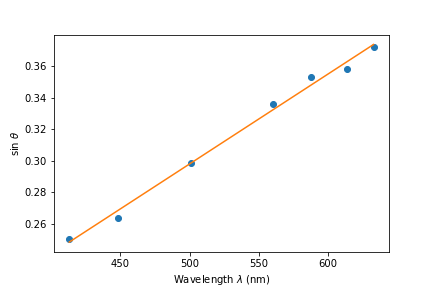
\includegraphics[scale = 0.56]{Figures/plot-1.png}
        \caption{The $Q \sim 1/I$ plot for $\nu_1$}
        \label{fig:plot1}
    \end{figure}
    \begin{figure}
        \centering
        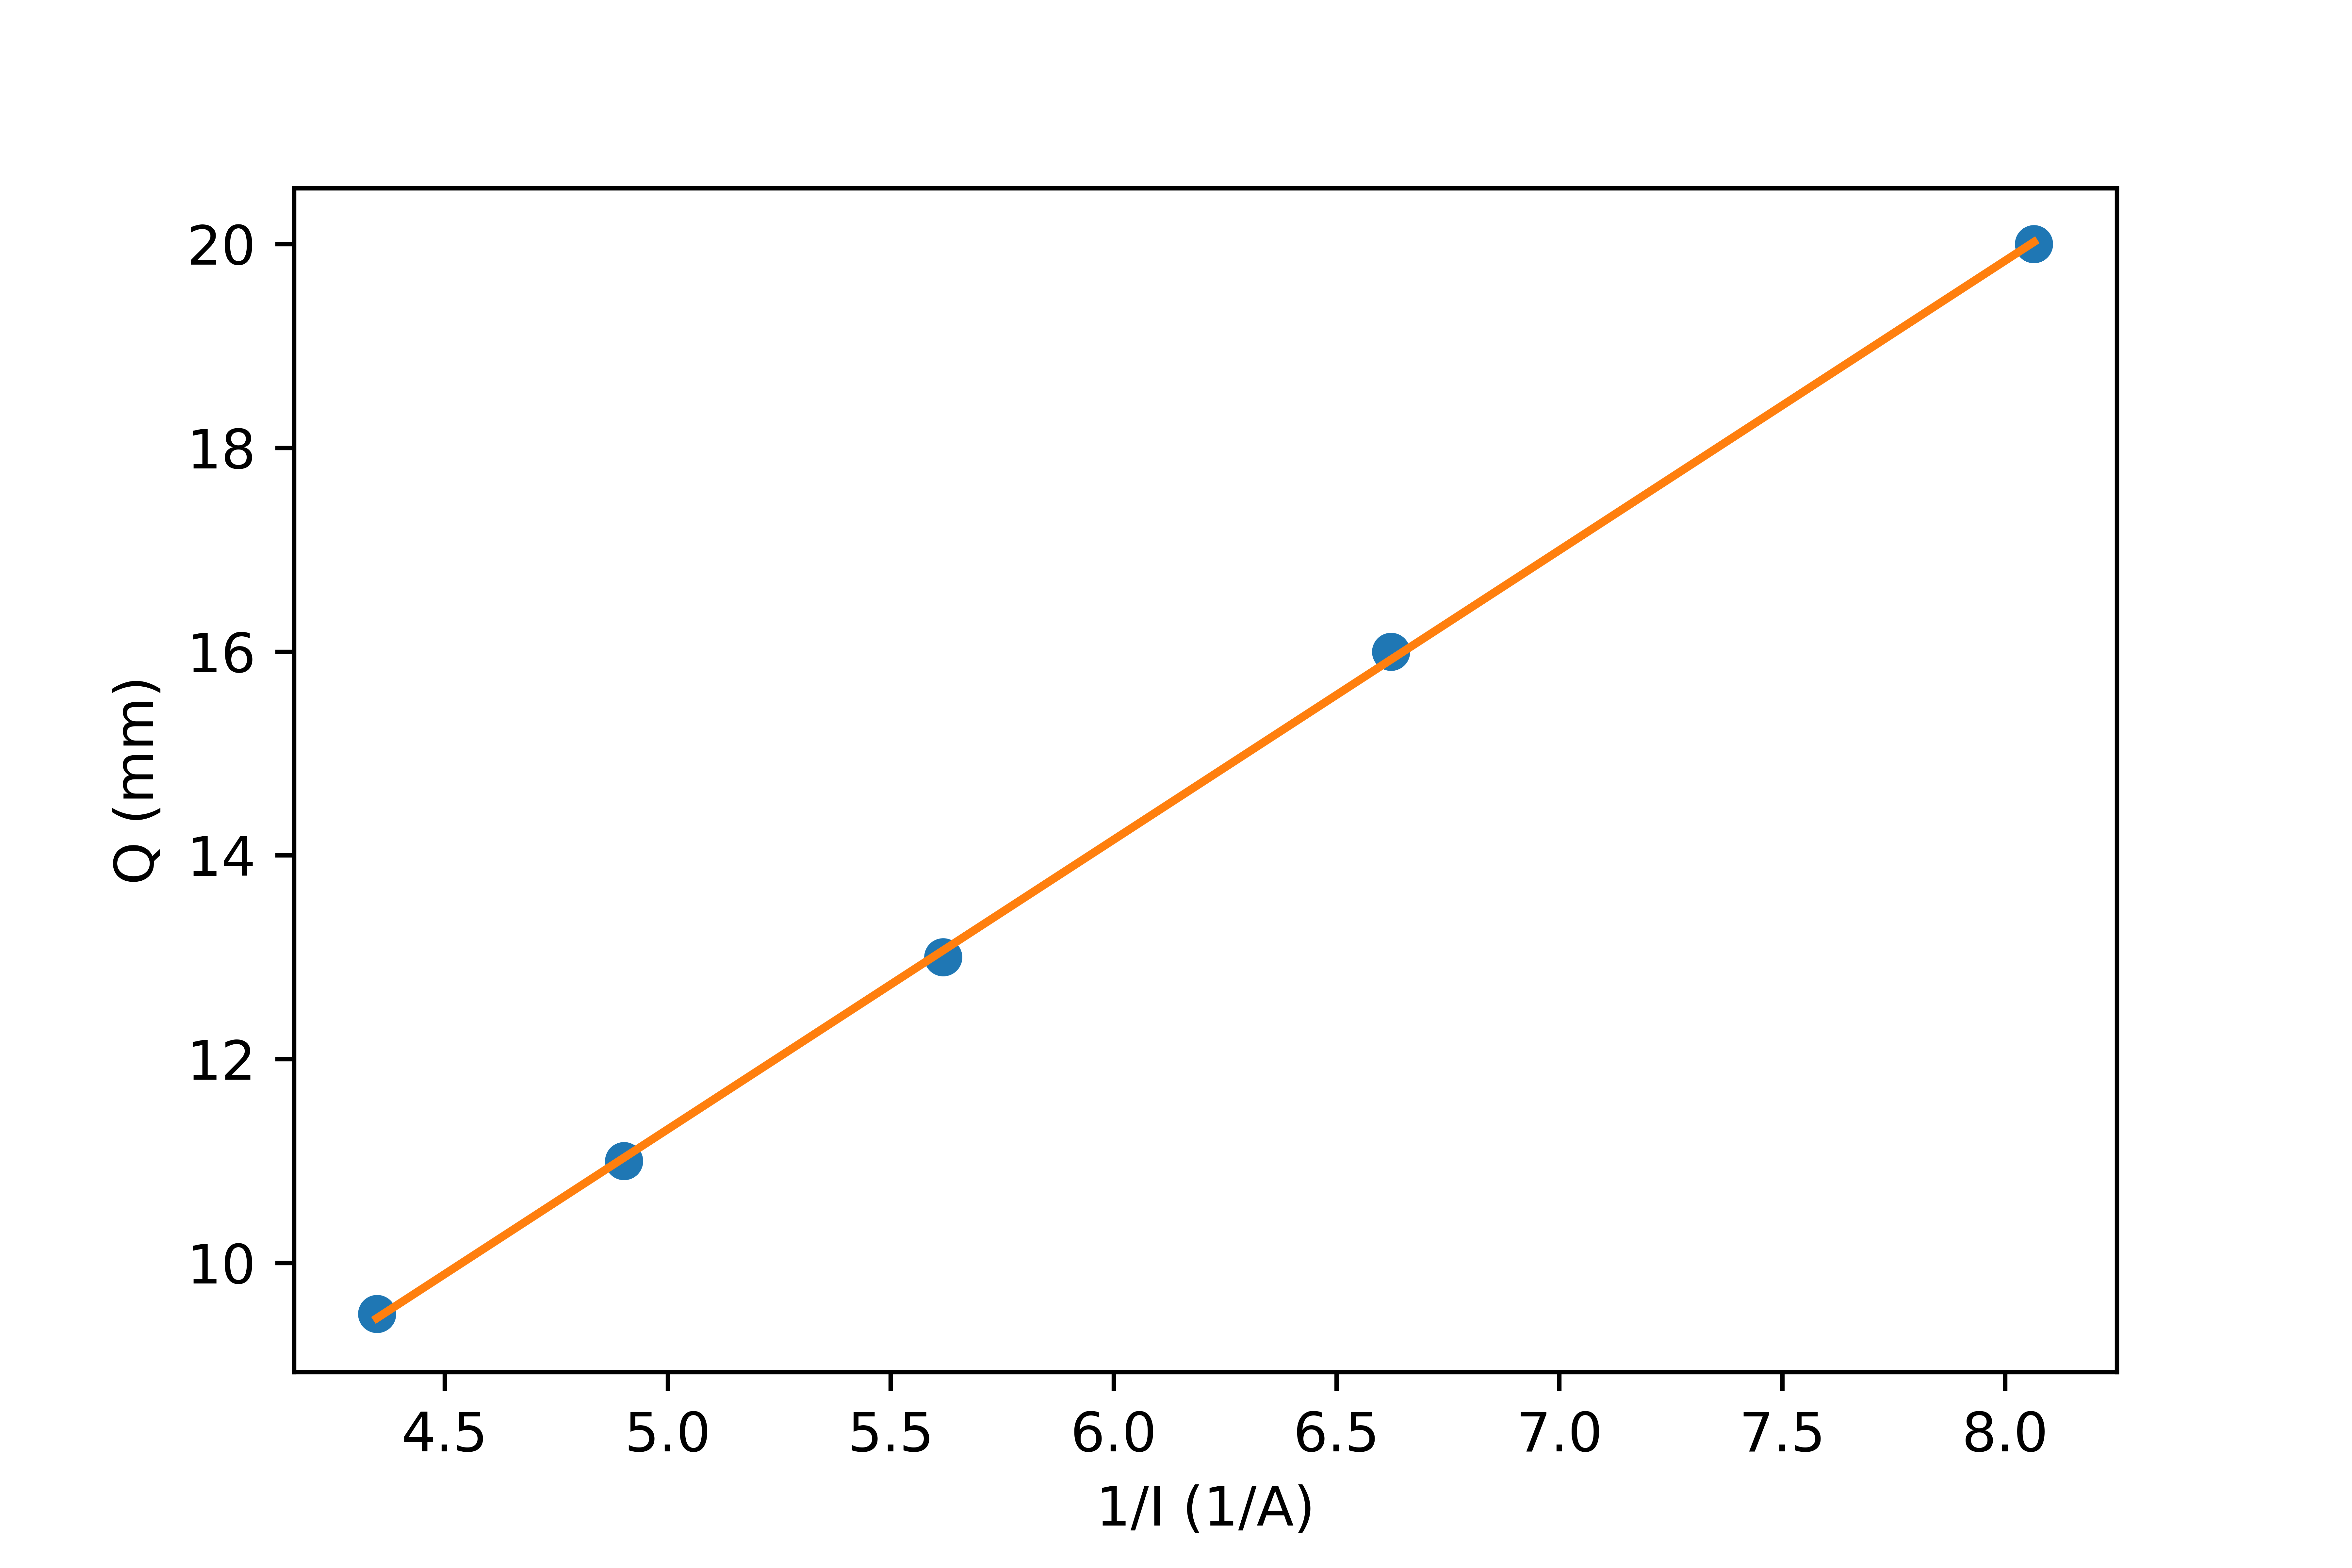
\includegraphics[scale = 0.56]{Figures/plot-2.png}
        \caption{The $Q \sim 1/I$ plot for $\nu_2$}
        \label{fig:plot2}
    \end{figure}

\section{Calculations and Results}
    We have from (\ref{eqDelE}) and (\ref{eqge}),
    \begin{equation}
    \label{eq26}
        g = \dfrac{h \nu}{\mu_B H_0}
    \end{equation}
    where $h = \SI{6.625e-27}{\erg \second}$, $\mu_B = \SI{0.927e-20}{\erg \per \gauss}$ and $H_0$ is magnetic field on the sample at the resonance. And from (\ref{eqH}), the magnetic field in at the centre of Helmholtz coils is
    \begin{equation}
        H = \dfrac{32 \pi n}{10 \sqrt{125} \cdot a} \cdot I \text{ gauss}
    \end{equation}
    Putting in the values, we get
    \begin{equation}
        H = 58.388 I \text{ gauss}
    \end{equation}
    As the peak to peak magnetic field is $H_{pp} = 2 \sqrt{2} H$, we have
    \begin{equation}
        H_{pp} = 165.146 I \text{ gauss}
    \end{equation}
    From here
    \begin{equation}
        H_0 = H_{pp} \dfrac{Q}{P} = 165.146 \dfrac{QI}{P}
    \end{equation}
    Now from (\ref{eqH0}), to find $QI$, we need the slope of curves plotted in figures (\ref{fig:plot1}) and (\ref{fig:plot2}).
    \par
    The five summations of for the data set plotted in figure (\ref{fig:plot1}) are as follows:
    \par
    \vspace{0.5cm}
    $S_{x} = \mathlarger{\mathlarger{\sum}} x_{i} = \SI{39.971}{\per \ampere}$, \hspace{0.5cm} $S_{y} = \mathlarger{\mathlarger{\sum}} y_{i} = \SI{66}{\milli \metre}$,
    \par
    \vspace{0.5cm}
    $S_{xx} = \mathlarger{\mathlarger{\sum}} x_{i}^2 = \SI{291.90}{\per \ampere \squared}$,
    \par
    \vspace{0.5cm}
    $S_{yy} = \mathlarger{\mathlarger{\sum}} y_{i}^2 = \SI{795.5}{\milli \metre \squared}$,
    \par
    \vspace{0.5cm}
    $S_{xy} = \mathlarger{\mathlarger{\sum}} x_{i}y_{i} = \SI{481.82}{\milli \metre \per \ampere}$.
    \par
    \vspace{0.5cm}
    Now the slope is given by,
    \begin{equation}
        m_{\nu_1} = \dfrac{S S_{xy} - S_{x}S_{y}}{S S_{xx} - S_{x}^2} = \SI{1.64539}{\milli \metre \ampere} = QI
    \end{equation}
    Now, putting in the values in (\ref{eq26}), we get 
        \begin{equation}
            \boxed{g_{\nu_1} = 1.97926} 
        \end{equation}
    Similarly for the five summations of for the data set plotted in figure (\ref{fig:plot2}) are as follows:
    \par
    \vspace{0.5cm}
    $S_{x} = \mathlarger{\mathlarger{\sum}} x_{i} = \SI{29.555}{\per \ampere}$, \hspace{0.5cm} $S_{y} = \mathlarger{\mathlarger{\sum}} y_{i} = \SI{69.5}{\milli \metre}$,
    \par
    \vspace{0.5cm}
    $S_{xx} = \mathlarger{\mathlarger{\sum}} x_{i}^2 = \SI{183.39}{\per \ampere \squared}$,
    \par
    \vspace{0.5cm}
    $S_{yy} = \mathlarger{\mathlarger{\sum}} y_{i}^2 = \SI{1036.25}{\milli \metre \squared}$,
    \par
    \vspace{0.5cm}
    $S_{xy} = \mathlarger{\mathlarger{\sum}} x_{i}y_{i} = \SI{435.51}{\milli \metre \per \ampere}$.
    \par
    \vspace{0.5cm}
    Now the slope is given by,
    \begin{equation}
        m_{\nu_2} = \dfrac{S S_{xy} - S_{x}S_{y}}{S S_{xx} - S_{x}^2} = \SI{2.84171}{\milli \metre \ampere} = QI
    \end{equation}
    Now, putting in the values in (\ref{eq26}), we get 
        \begin{equation}
            \boxed{g_{\nu_2} = 1.25532}
        \end{equation}
    



    

\section{Error Analysis}
    Error in $g$ is given by
    \begin{equation}
    \label{eqerrorg}
        dg = \sqrt{\Big(\dfrac{\partial g}{\partial \nu} \sigma_{\nu}\Big)^2 + \Big(\dfrac{\partial g}{\partial P} \sigma_{P}\Big)^2 + \Big(\dfrac{\partial g}{\partial m} \sigma_{m}\Big)^2}
    \end{equation}
    where $m$ and $\sigma_m$ represent the slope and error in slope respectively. Now error in slope is given by
    \begin{equation}
    \label{eqslope}
        \sigma_m = \sigma_y \times \sqrt{\dfrac{S}{\Delta}}
    \end{equation}
    $\sigma_y$ is the uncertainty in the measurement of $Q$ which is equal to its least count of measurement $\SI{2}{\milli \metre}$ and $\Delta = S S_{xx} - S_x^2$. Putting in the values in equations (\ref{eqerrorg}) and (\ref{eqslope}) and solving, we get
    \begin{equation}
        \boxed{d g_{\nu_1} = 0.5}
    \end{equation}
    and
    \begin{equation}
        \boxed{d g_{\nu_2} = 0.3}
    \end{equation}

        



\section{Discussions}
\begin{enumerate}
    \item Note that the frequencies used in magnetic resonance experiments range from $10^9$ to $10^{11}$ cps. These frequencies situated below the limits of the infrared part of the spectrum, allow highly accurate investigation of energy level splitting so small that they are inaccessible or almost inaccessible by optical methods. 
    \item The probability of spontaneous transition in the radio-frequency region is very small, since this probability is proportional to $\nu^3$. Therefore, in paramagnetic resonance studies one is forced to deal only with induced absorption and emission. 
    \item While in the great majority of cases optical spectra arise from electric dipole transitions between energy levels, the lines of paramagnetic resonance absorption arise exclusively from magnetic dipole transitions. Consequently, the Einstein coefficients for induced absorption and emission will, in the case of paramagnetic resonance, be smaller by roughly four orders of magnitude.
    \item As a result, the paramagnetic resonance effect is exceedingly small; if it can be observed at all is due to the high sensitivity of electronic methods of detection and the enormous number of photons coming into play ($\SI{1}{\milli \watt}$ corresponds to $n \simeq 10^{20}$ photons per sec at a frequency of $10^{10}$ cps). 
    \item In the optical frequency region the line width is always very small in comparison with the fundamental frequency. In paramagnetic resonance the relation between these quantities becomes quite different, since the interactions causing a broadening of the lines can be of the same order of magnitude as the energy splitting which determines the resonance frequency. Because of this the width of paramagnetic resonance lines is often comparable to the fundamental frequency and can be measured with great accuracy. This opens up wide possibilities for investigation of different types of interactions in paramagnetic substances by means of analysis of the shape and width of a paramagnetic resonance line and of the character of its dependence upon various factors. 
    \item The most important factors determining the line width are magnetic dipole interactions, exchange forces, local electrical fields created by neighbouring magnetic particles, and finally, thermal motion; the natural line widths of radio- frequency spectra are completely negligible. 
    \item In contrast with optical experiments, in radio-frequency spectroscopy it is customary to use radiation which is so monochromatic that the generated band of frequencies is incomparably narrower than the absorption line width. 
    \item Paramagnetic resonance spectra are not studied by varying the frequency of the incident radiation, but by varying the characteristic frequencies of the absorbing systems. This is achieved by varying the static magnetic field.
    \item That is ESR can be observed at radio frequencies in a magnetic field of few gauss or otherwise in the microwave region in a magnetic field of a few kilogauss. The latter alternate has many distinct advantages like for each transition the absorbed energy is much larger, and thus the signal-to-noise ratio is much improved and a high magnetic field is used, thus providing separation between levels that are intrinsically wide and would remain partially overlapped at low fields. Because of these advantages, ESR in microwave region is preferred for research purposes. 
    \item The observed peaks are in fact absorption dips, because the sample absorb power from the induction coil. The spin precesses with Larmor's frequency $\omega_0$ and hence varies in magnitude and direction due to variation of magnetic field $\Vec{H_0}$ which is due to an alternating current in the Helmholtz coils. Now if the radio frequency field, $\omega_1$ falls in the range of $\omega_0$ the resonance occurs
    \item The coincidence of peaks on the $x$-scale needs to be calibrated for magnetic field measurements. The coincidence ensures that the magnetic field is zero at the centre and has the peak values at the two ends. Complete merger of the peaks on $y$-scale may not occur due to many reasons such as $\SI{50}{\hertz}$ pick-ups, ripples in the power supply etc. Though, every effort has been made to minimise these factors but the large amplification ($\simeq 4000$) in the circuitry make them substantial. However, any non- coincidence on the $y$-scale is immaterial as neither any measurement of the $y$-scale is involved in the calculation of $g$-factor nor any measurement is made on it.
    \begin{figure}
        \centering
        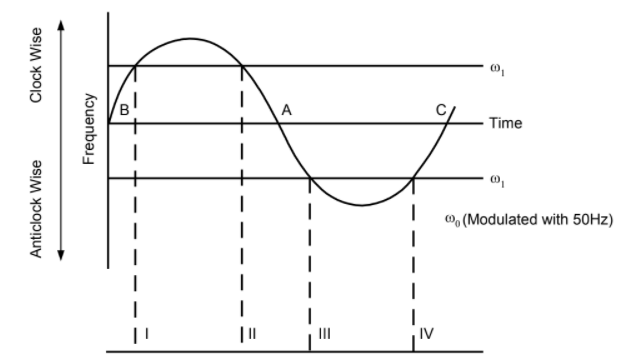
\includegraphics[scale = 0.65]{Figures/radfreq.png}
        \caption{The radio frequency is linear by polarised, which can be regarded as two circularly polarised fields of opposite direction (say clockwise and anti clockwise). Further magnetic field $H_0$ also changes direction. Thus resonance occurs when the two frequencies ($\omega_1$ and $\omega_0$) becomes equal in magnitude as well as direction i.e. four times in one full cycle of $H_0$.}
        \label{fig:radfreq}
    \end{figure}
    \begin{figure}
        \centering
        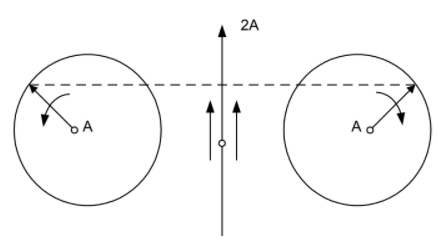
\includegraphics[scale = 0.8]{Figures/linfreq.png}
        \caption{A linearly field of frequency is equivalent to two fields rotating in opposite direction with the same frequency $\omega$}
        \label{fig:linfreq}
    \end{figure}
\end{enumerate}

\section{Conclusions}
\begin{enumerate}
    \item The value of $g$-factor for $\nu_1 = \SI{13.05}{\mega \hertz}$ was found to be $g = 2.0 \pm 0.5$ after taking care of the significant figures.
    \item The value of $g$-factor for $\nu_2 = \SI{14.72}{\mega \hertz}$ was found to be $g = 1.2 \pm 0.3$ after taking care of the significant figures. 
    \item Although the first value was obtained very close to the literature value, the value for second frequency was unsatisfactory.
    \item The results so obtained were in the order of the expected values for the lower frequency. The experiment was thus a moderate success.
\end{enumerate}




% Produces the bibliography via BibTeX.

\end{document}
%
% ****** End of file apssamp.tex ******
